\paragraph*{High inertial effects :}
We now turn our attention to the high inertial regime for which we set $Ga =100$.
In this situation it is expected that the presence of wake change completely the flow behavior. 
\begin{figure}[h!]
    \centering
    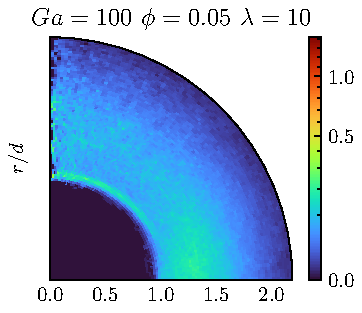
\includegraphics[height=0.2\textwidth]{image/HOMOGENEOUS_NEW/Dist/Pnst_l_10_Ga_100_PHI_0_05.pdf}
    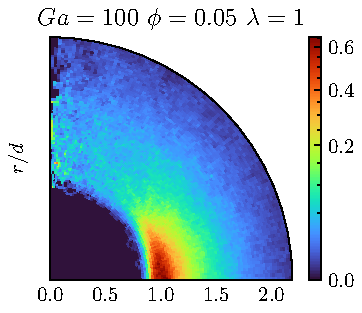
\includegraphics[height=0.2\textwidth]{image/HOMOGENEOUS_NEW/Dist/Pnst_l_1_Ga_100_PHI_0_05.pdf}
    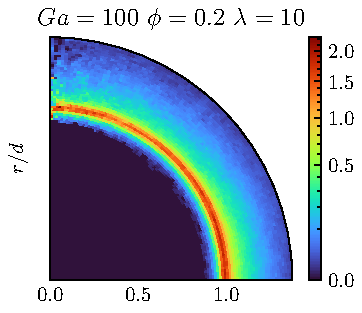
\includegraphics[height=0.2\textwidth]{image/HOMOGENEOUS_NEW/Dist/Pnst_l_10_Ga_100_PHI_0_2.pdf}
    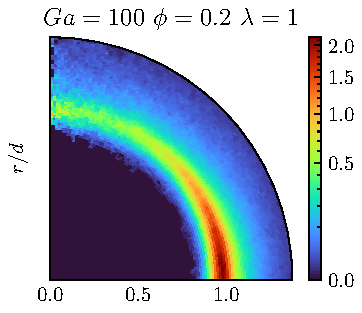
\includegraphics[height=0.2\textwidth]{image/HOMOGENEOUS_NEW/Dist/Pnst_l_1_Ga_100_PHI_0_2.pdf}
    \caption{Histogram of the probability density function $P_\text{nst}$ at high inertial effect $Ga = 100$.
    (left) Low volume fraction cases $\phi=0.05$ for $\lambda = 1,10$.
    (right) High volume fraction cases $\phi=0.1$ for $\lambda = 1,10$ }
    \label{fig:Pnst_high_Ga}
\end{figure}
As expected, if we compare \ref{fig:Pnst_high_Ga} (right) with their corresponding cases from \ref{fig:Pnst_low_Ga} (right) we observe that the nearest PDF becomes even more concentrated at contact of the particles for $Ga=100$.
In general, if we compare all PDF from the low inertial cases to these, the striking difference is the presence of anisotropy in \ref{fig:Pnst_high_Ga}. 
Especially, even within the high inertial cases we can notice that the PDF is even more concentrated on the sides for $\lambda = 1$. 
Consequently, it is clear that the PDF concentration on the side increase for increasing $Ga$ and for low viscosity ratio. 
Regarding, the volume fraction it is found to decrease the anisotropy but makes the particles closer. 

To illustrate the influence of teh viscosity ratio on the microstructure \ref{fig:images} displays snapshots of two DNS at $\phi = 0.05$ and $Ga = 100$. 
As predicted by $P_\text{nst}$ in \ref{fig:Pnst_high_Ga} we observe strong layers of droplets for $\lambda = 1$ in opposition to the viscous droplets which are more evenly dispersed. 
\begin{figure}[h!]
    \centering
    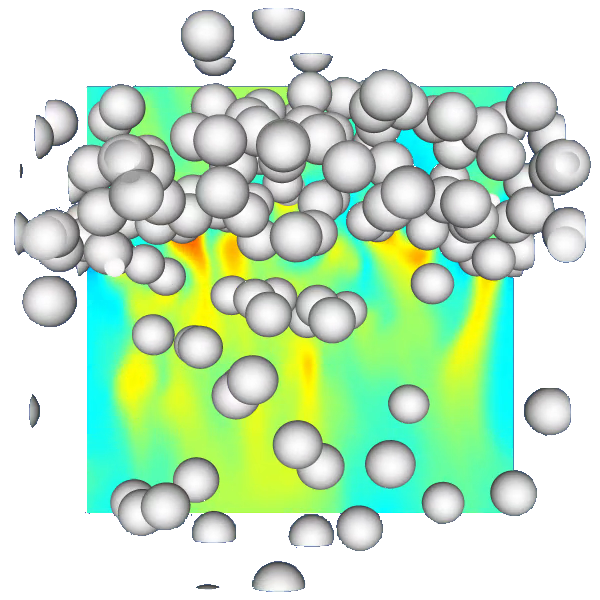
\includegraphics[width=0.35\textwidth]{image/HOMOGENEOUS_NEW/P_PHI_5_l_10_Ga_100.png}
    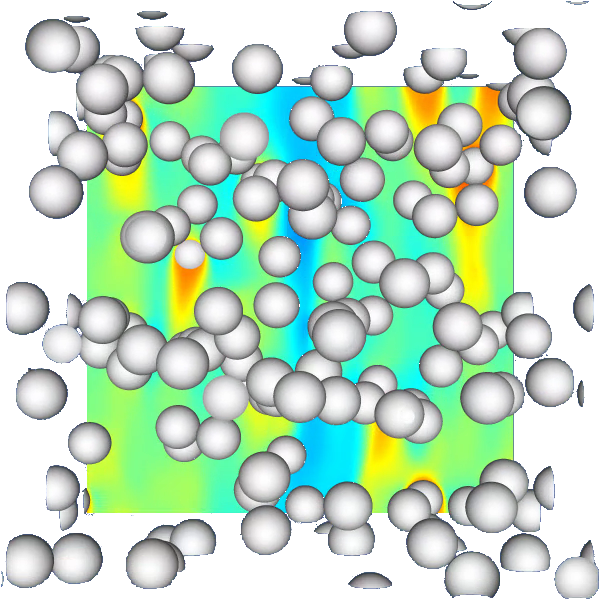
\includegraphics[width=0.35\textwidth]{image/HOMOGENEOUS_NEW/P_PHI_5_l_1_Ga_100.png}
    \caption{Snapshot of a simulation at $t^* = 150$ for $\phi=0.05$ and $Ga=100$.
    Color map : values of the vertical component of the velocity, field on the vertical plane defined by the equation $z=0$. 
    (left)  $\lambda = 1$.
    (right)  $\lambda = 10$.
    }
    \label{fig:images}
\end{figure}
Clearly, the viscosity ratio appears to maintain a significant distance between particles, which prevent the creation of structures such as droplets layers. 
Nevertheless, we can observe on \ref{fig:images}(left) that the length between the layers is roughly equal to the length of the numerical domain. 
Indeed, only one layer of droplets is present in the domain. 
Therefore, at this stage it is hard to known for sure if the current microstructure is constrained by the size of the numerical domain, or if it is well representative of the actual microstructure that we would obtain in an infinite non-periodic domain. 
Consequently, in all rigor DNS in a larger domain would be required to evaluate the microstructure dependence on the domain size. 
It is clear that DNS in a larger domain with the same dimensionless parameters are expensive therefore it has not been conducted in this study. 
For now, the only conclusion from  \ref{fig:images} that we are able to make is : more cluster are formed at $\lambda =1$ than at $\lambda = 10$, however we cannot be sure that the cluster are realistic in the former case.



Although, \ref{fig:Pnst_high_Ga} and \ref{fig:Pnst_low_Ga} give a good representation of the particle pair azimuthal distribution, it is hard to inspect in details the radial distribution.
Therefore, in \ref{fig:Pr}  we plotted the radial distribution $P_\text{nst}(r)$ for two different viscosity ratios and multiples \textit{Galileo} numbers in terms of the dimensionless distance $(r - d)/d_p$ where $d_p$ is the mean particle distance defined as $d_p = n_p^{-1/3}$.  
\begin{figure}[h!]
    \centering
    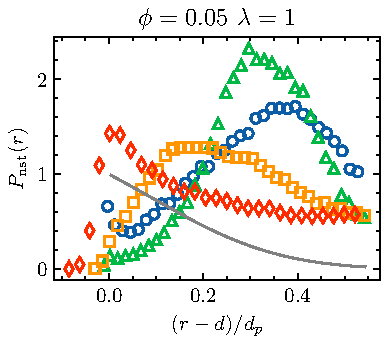
\includegraphics[height=0.35\textwidth]{image/HOMOGENEOUS_NEW/Dist/Pr_l_1_PHI_5.pdf}
    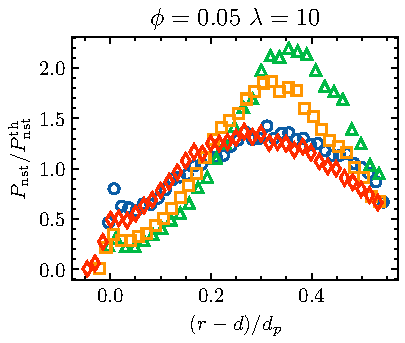
\includegraphics[height=0.35\textwidth]{image/HOMOGENEOUS_NEW/Dist/Pr_l_10_PHI_5.pdf}
    \caption{Radial probability density function $P_\text{nst}(|r|)$ in terms of the dimensionless distance $(r-d)/d_p$ where, $d_p = n_p^{-1/3}$, for  $\phi = 0.05$.
    (left)  $\lambda = 1$.
    (right) $\lambda = 10$.
    ($\circ$)  $Ga = 10$ 
    ($\triangle$)  $Ga = 25$ 
    ($\square$)  $Ga = 50$ 
    ($\lozenge$)  $Ga = 100$ 
    (grey Solid lines) Theoretical distribution valid for dilute dispersion of randomly distributed hard spheres, defined \ref{eq:Pnst_dilute}.
    }
    \label{fig:Pr}
\end{figure}
The radial distribution seem concentrated in different zones with varying \textit{Galileo} number when $\lambda = 1$, see \ref{eq:Pr}(left), while the distribution seem rather unchanged with multiples \textit{Galileo} numbers for $\lambda = 10$ \ref{fig:images}(right). 
In both cases the radial distribution does not follow the random hard sphere distribution defined by \ref{eq:Pnst_dilute}. 
Far from the particle the distribution seem tangent to it 
It is clear that when inertial effects are strong, the viscosity ratio $\lambda$ has an important impact on the radial distribution. 
Indeed, we can notice the remarkable difference between \ref{fig:Pr}(left) and  \ref{fig:Pr}(right) at $Ga = 100$ ($\lozenge$ symbols). 
For $\lambda = 1$ the distribution at $Ga = 100$ is high at the contact of the particles $(r-d)/d_p = 0$. 
In fact, it is not surprising when considering the high particle density zone formed by the cluster, see \ref{fig:images}(left). 
In opposition, for $\lambda  = 10$ the radial distribution it is completely different, the particles are in averaged further away form each other, as it could be predicted from \ref{fig:images}(right).
Additionally, the effect of the \textit{Galileo} number on $P_\text{nst}(r)$ doesn't seem important contrasting with the low viscosity ratio cases where it has a major influence.  

In short, we observed that both, the radial and azimuthal distribution were affected by the inertial effect measured by the \textit{Galileo} number. 
The major effect coming with high inertia is the generation of strong anisotropy in the particle pair distribution. 
Regarding the viscosity ratio, it has a strong impact on the emulsion distribution, however, this is only true at high $Ga$ whereas at low $Ga$ the change in viscosity ratio has no notable impact. 
Furthermore, low viscosity ratio generate anisotropy in the distribution.  
Additionally, it is seen that the particle distribution gets more concentrated at the contact of the test sphere, but only for $\lambda = 1$. 

Therefore, in the following we try to explain the origin of the striking difference between $\lambda = 1$ and $\lambda = 10$ on the distribution.
With this objectif in mind, we present in the following section a meticulous analysis of the relative average particles' velocity. 


\tb{Explain the implication of the on the forces fits}

\tb{The dead zone at the top and the accumulation at contact of the particle is clearly present at $Ga=50$ and disapear at $Ga=100$ it might be interesting to mention that just like in \citet{seyed2021sedimentation}.}
\tb{We are clearly below the Galileo where $\phi$ gets a high zone above}

\tb{The dead zone at low $\phi$ becomes a high zone \citet{shajahan2023inertial,seyed2021sedimentation}}

\tb{The anisotropisation with $\phi$ is clearly mentioned in these studies}


\tb{The isotropisation at high Galile might be explain with the Pnorm which randomize \citet{shajahan2023inertial}}